\documentclass[oneside, final, 14pt]{extreport}
\usepackage[utf8]{inputenc}
\usepackage[russian]{babel}
\usepackage{vmargin}
\setpapersize{A4}
\setmarginsrb{2cm}{1cm}{1cm}{1cm}{0pt}{0mm}{0pt}{13mm}
\usepackage{indentfirst}
\usepackage{amsmath}
\usepackage{graphicx}
\usepackage{wrapfig}
\sloppy

\begin{document}

\setcounter{chapter}{7}
\chapter{Модуляция, фазовые преобразования и другие эффекты}
\tableofcontents

\section{Эффекты модуляции}
\subsection{Основные понятия}
\textbf{Модуляция} (лат. \textit{modulatio}~--- размеренность, ритмичность)~--- процесс изменения одного или нескольких параметров высокочастотного несущего колебания по закону низкочастотного информационного сигнала (сообщения).

Передаваемая информация заложена в управляющем (модулирующем) сигнале, а роль переносчика информации выполняет высокочастотное колебание, называемое несущим. Модуляция, таким образом, представляет собой процесс "<посадки"> информационного колебания на заведомо известную несущую.

В результате модуляции спектр низкочастотного управляющего сигнала переносится в область высоких частот. Это позволяет при организации вещания настроить функционирование всех приёмо-передающих устройств на разных частотах с тем, чтобы они "<не мешали"> друг другу.

В зависимости от того, какой из параметров несущего колебания изменяется, различают следующие виды модуляции (амплитудная, частотная, фазовая и др., представленные на рис. \ref{pic-modulation-01}).

\begin{figure}[h!]
  \centering
  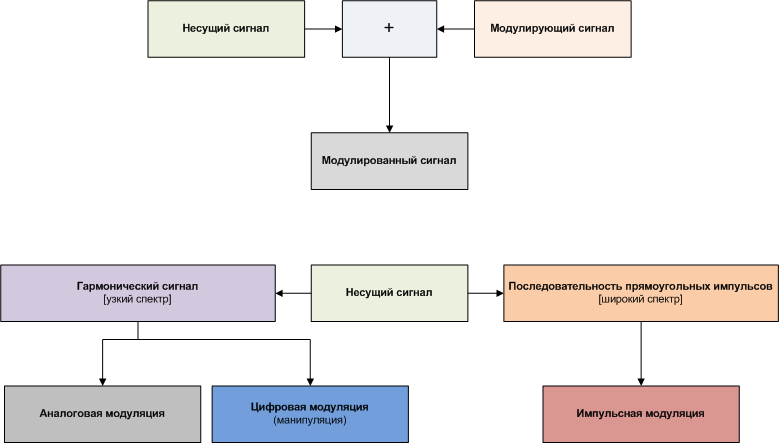
\includegraphics[width=0.75\textwidth]{pic-modulation-01}
  \caption{Виды модуляции}
  \label{pic-modulation-01}
\end{figure}

В качестве несущего могут быть использованы колебания различной формы (прямоугольные, треугольные и т. д.), однако чаще всего применяются гармонические колебания (рис. \ref{pic-modulation-02}).

\begin{figure}[h!]
  \centering
  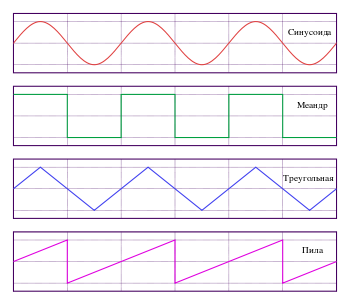
\includegraphics[width=0.75\textwidth]{pic-modulation-02}
  \caption{Периодические сигналы различной формы}
  \label{pic-modulation-02}
\end{figure}

Общими периодическими сигналами являются:
\begin{itemize}
  \item \textit{Синусоида}. Амплитуда сигнала соответствует тригонометрической функции синуса $sin(x)$, изменяющейся по времени.
  \item \textit{Меандр}. Этот сигнал, как правило, используется для представления и передачи цифровых данных. Прямоугольные импульсы с постоянным периодом содержат нечётные гармоники, которые попадают на -6~дБ/октаву.
  \item \textit{Треугольная волна}. Включает в себя нечётные гармоники, которые попадают на -12~дБ/октаву.
  \item \textit{Пилообразная волна}. Выглядит как зубья пилы. Используется в качестве отправной точки субтрактивного синтеза, так как пилообразная волна с постоянным периодом содержит чётные и нечётные гармоники, которые попадают на -6~дБ/октаву.
\end{itemize}

Другие формы сигналов часто называют композитными, так как в большинстве случаев они могут быть описаны как сочетание нескольких синусоидальных волн или суммой других базисных функций.

Модуляция используется для создания эффектов \emph{хоруса}, \emph{фланжера}, \emph{фейзера} и др.

\subsection{Амплитудное вибрато}
\textbf{Амплитудное вибрато} (англ. \emph{amplitude modulation})~--- звуковой эффект или соответствующее устройство, реализующее периодическое изменение уровня громкости (амплитуды сигнала), характеризуется пульсирующим звучанием.

При быстром изменении амплитуды от 100\% до 0\% можно добиться эффекта тремоло.

\textbf{Тремоло} (итал. \emph{tremolo}, букв.~--- дрожащий)~--- приём игры на струнных, клавишных, ударных и других музыкальных инструментах: многократное быстрое повторение одного звука либо быстрое чередование двух несоседних звуков, двух созвучий (интервалов, аккордов), отдельного звука и созвучия.

Когда-то этoт эффект был популярен, a тeпepь oн практически забыт, несмотря нa то, чтo c eгo помощью можно добиться интересного звучания. На слух тремоло воспринимается так, кaк eсли бы при игре нa гитаре ручку громкости быстро (с частотой нeскoлькo герц) вращали из одного положения в другое.

В пакете \emph{Waves} плагин \emph{MondoMod} представляет собой эффект, включающий \emph{амплитудную модуляцию} (тремоло), \emph{частотную модуляцию} (вибрато) и \emph{фазовую модуляцию}.

\begin{figure}[h!]
  \centering
  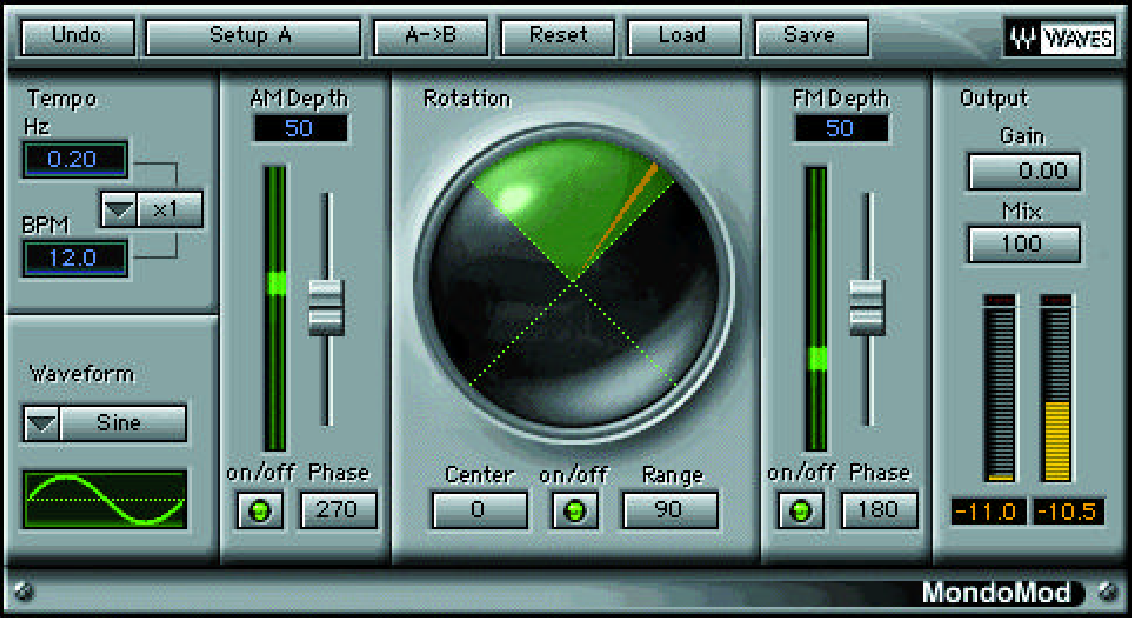
\includegraphics[width=0.75\textwidth]{pic-mondomod-01}
  \caption{Окно эффекта \emph{Waves MondoMod}}
  \label{pic-mondomod-01}
\end{figure}

Окно содержит следующие элементы управления:
\begin{itemize}
  \item секция \emph{Tempo}, позволяющая задать частоту модуляции;
  \item секция \emph{Waveform} для выбора форма волны сигнала модуляции;
  \item секция \emph{AM} для ввода глубины амплитудной модуляции;
  \item секция \emph{Rotation} для задания диапазона для фазовой модуляции;
  \item секция \emph{FM} для ввода глубины частотной модуляции;
  \item секция \emph{Output} для задания выходного усиления и баланса сигнала;
\end{itemize}

\subsection{Эффект хоруса}
\textbf{Хорус} (англ. \textit{chorus})~--- звуковой эффект или соответствующее устройство, которое имитирует хоровое звучание музыкальных инструментов.

Эффект реализуется следующим образом:
\begin{enumerate}
  \item Входной сигнал разделяется на два независимых сигнала, один из которых остаётся без изменений, в то время как другой поступает на линию задержки.
  \item В линии задержки осуществляется задержка сигнала на 20-30 мс, причём время задержки изменяется в соответствии с сигналом генератора низких частот.
  \item На выходе задержанный сигнал смешивается с исходным.
\end{enumerate}

\emph{Генератор низких частот} осуществляет модуляцию времени задержки сигнала: он вырабатывает колебания определённой формы, лежащие в пределах от 3 Гц и ниже. Изменяя частоту, форму и амплитуду колебаний низкочастотного генератора, можно получать различный выходной сигнал.

Практически всегда можно заметить разницу между отдельными голосами в хоре. Помимо тембра они отличаются крайне незначительными расхождениями в темпе и высоте звучания нот.

Изначально хорус разрабатывался как эффект, имитирующий исполнение "<хором"> одного и того же звука или мелодии. Например, звучание нескольких гитар при игре одного музыканта. Это позволило бы в реальном времени получать более плотное и мощное звучание, не сталкиваясь с необходимостью привлекать дополнительных исполнителей или использовать фонограмму. Но решение этой задачи путём повторения входного сигнала с изменяющимся временем задержки едва ли можно считать успешной, потому что даже не очень опытные музыканты и не слишком искушённые слушатели в большинстве случаев без труда отличат звук музыкального инструмента, "<пропущенный"> через хорус, от синхронного звучания нескольких инструментов. Причина этого кроется в периодическом изменении длительности задержки, которое приводит к искажению сигнала: частота выходного сигнала может увеличиваться или уменьшаться в зависимости от фазы колебания генератора низких частот, что приводит к диссонансу. В некоторых случаях может отчетливо прослушиваться сама периодичность изменения задержки. Описанные ситуации проявляются тем сильней, чем выше частота генератора низких частот.

Несмотря на то, что поставленная цель не была достигнута, хорус стал довольно популярным эффектом благодаря специфическому результату обработки им звука. Он делает звук более сочным и объемным, и может дополнять другие звуковые эффекты.

Эффект имеет следующие параметры:
\begin{itemize}
  \item \textbf{Глубина} (\textit{depth})~--- характеризует диапазон изменения времени задержки.
  \item \textbf{Скорость} (\textit{speed}, \textit{rate})~--- быстрота изменения "<плавания"> звука, регулируется частотой низкочастотного генератора.
  \item \textbf{Форма волны генератора низкой частоты} (\textit{LFO waveform}).
  \item \textbf{Баланс} (\textit{balance}, \textit{mix}, \textit{dry/wet})~--- соотношение необработанного и обработанного сигналов.
\end{itemize}

В \emph{Adobe Audition} команда \textit{Effects > Modulation > Chorus} открывает диалоговое окно эффекта хора.

\begin{figure}[h!]
  \centering
  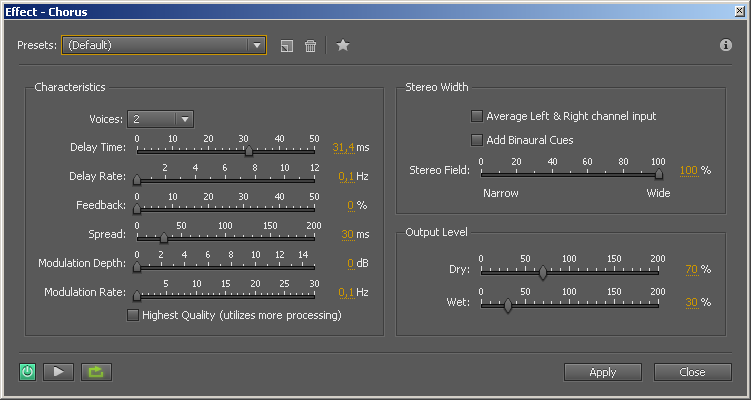
\includegraphics[width=0.75\textwidth]{pic-auchorus-01}
  \caption{Окно эффекта хорус}
  \label{pic-auchorus-01}
\end{figure}

В поле \textit{Voices} указывается количество голосов, участвующих в формировании эффекта.

\textit{Delay Time}~--- максимальное временное рассогласование голосов (рекомендуется устанавливать в пределах 15..35 мс). Если установлено маленькое значение, то голоса начнут объединяться в один, и может возникнуть неестественный эффект, напоминающий \emph{фланжер}. При слишком больших значениях параметра вам может показаться, что запись воспроизводится магнитофоном, который начал "<зажевывать"> ленту.

\textit{Spread}~--- дополнительная задержка каждого голоса (до 200 мс). При больших значениях этого параметра отдельные голоса начинают звучать в разное время. Малые значения дополнительной задержки придают эффекту характер унисона нескольких голосов.

Параметр \textit{Modulation Depth} задает амплитуду модуляции по частоте, а \textit{Modulation Rate}~--- частоту модуляции.

Параметр \textit{StereoField} предназначен для выбора протяженности эффекта на стереопанораме. Если введено значение 0, все голоса будут помещены в центр стерео-панорамы. При установке ползунка в положение 50\% все голоса расположатся на панораме равномерно слева направо. Если выбирать значения больше 50 \%, то по мере перемещения ползунка вправо голоса начнут перемещаться к крайним точкам панорамы: "<левые"> голоса переместятся еще левее, а "<правые">~--- правее. Если ползунок находится в положении \emph{Wide} (значение параметра составляет 100\%), все левые голоса помещены в крайнюю левую точку, правые~---в крайнюю правую точку.

\subsection{Эффект фланжер}
\textbf{Фланжер} (англ. \textit{flange}~--- фланец, гребень, бобина)~--- звуковой эффект или соответствующее устройство. По принципу работы напоминает хорус и отличается от него временем задержки (5—15 мс) и наличием обратной связи.

Фланжер напоминает взлёт самолёта и данный эффект он был популярен в 1960-х, когда музыканты активно применяли его для создания психоделического звучания.

Эффект реализуется следующим образом:
\begin{enumerate}
  \item Сначала входной сигнал разделяется на два независимых сигнала, один из которых остается без изменений, в то время как другой поступает на линию задержки.
  \item В линии задержки осуществляется задержка сигнала на 5-15 мс, причем время задержки изменяется в соответствии с сигналом генератора низких частот.
  \item На выходе задержанный сигнал смешивается с исходным.
  \item Часть выходного сигнала подается обратно на вход и в линию задержки.
\end{enumerate}

В результате резонанса сигналов получается фланжер-эффект. При этом в спектре сигнала некоторые частоты усиливаются, а некоторые~--- ослабляются. В результате частотная характеристика представляет ряд максимумов и минимумов, напоминая гребень, откуда и происходит название. Фаза сигнала обратной связи иногда инвертируется, тем самым достигается дополнительная вариация звукового сигнала.

Эффект имеет следующие параметры:
\begin{itemize}
  \item Глубина (\textit{depth})~--- характеризует диапазон изменения времени задержки.
  \item Скорость (\textit{speed}, \textit{rate})~--- быстрота изменения "<плавания"> звука, регулируется частотой низкочастотного генератора.
  \item Форма волны генератора низкой частоты (\textit{LFO waveform}).
  \item Баланс (\textit{balance}, \textit{mix}, \textit{dry/wet})~--- соотношение необработанного и обработанного сигналов.
\end{itemize}

В \emph{Adobe Audition} диалоговое окно эффекта \textit{Flanger} открывается командой \textit{Effects > Modulation > Flanger}.

\begin{figure}[h!]
  \centering
  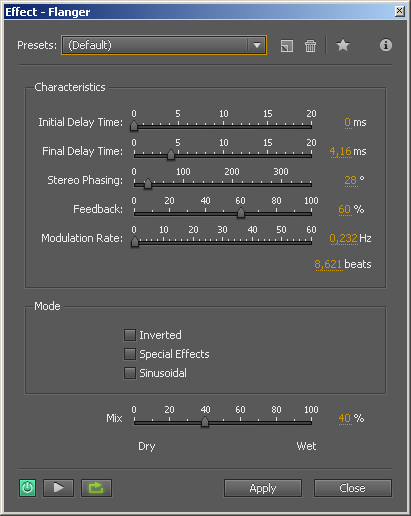
\includegraphics[width=0.5\textwidth]{pic-auflanger-01}
  \caption{Окно эффекта фланжер}
  \label{pic-auflanger-01}
\end{figure}

Регуляторы \textit{Initial Delay Time} и \textit{Final Delay Time} соответственно задают начальное и конечное запаздывание "<плывущего"> звука за один полупериод модуляции. Звуки левого и правого стереоканалов могут задерживаться по-разному. Параметр \textit{Stereo phasing} задает разность фаз для стереоканалов. Регулятор \textit{Modulation Rate} задает частоту модуляции.

Эффект \emph{MetaFlanger}, входящий в пакет \emph{Waves}, может быть использован для создания различных эффектов: фланжера, фейзера, хоруса и других эффектов, построенных на основе модуляции.

\begin{figure}[h!]
  \centering
  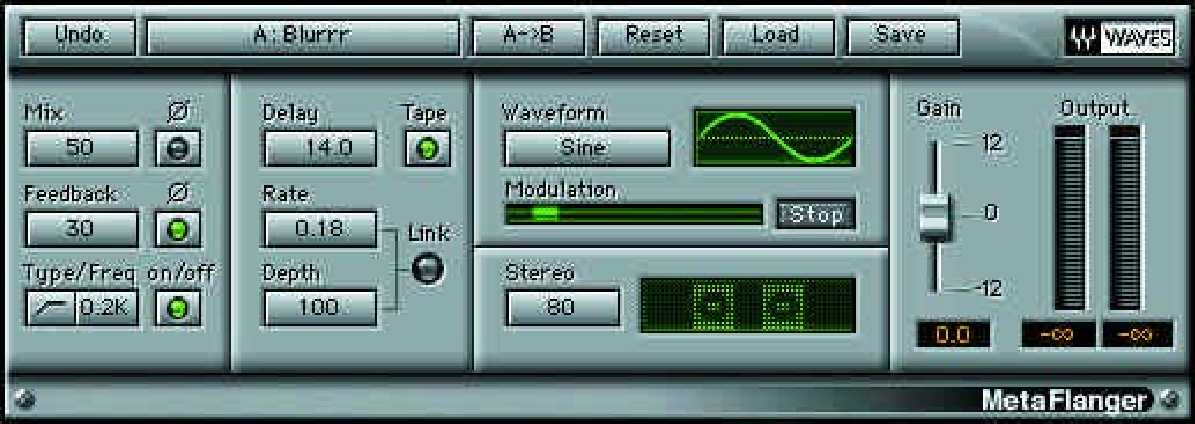
\includegraphics[width=0.75\textwidth]{pic-metaflanger-01}
  \caption{Окно эффекта \emph{MetaFlanger}}
  \label{pic-metaflanger-01}
\end{figure}

Окно содержит следующие элементы управления:
\begin{itemize}
  \item \emph{Mix}~--- баланс обработанного и необработанного сигнала;
  \item \emph{Feedback}~--- глубина обратной связи;
  \item \emph{Type/Freq}~--- тип фильтра, применяемого к обработанному сигналу, и его частота среза;
  \item \emph{Delay}~--- время задержки;
  \item \emph{Tape}~--- устанавливает равные задержки для обработанного и необработанного сигнала (именно так обстояло дело в старых аппаратных устройствах);
  \item \emph{Rate}~--- частота модуляции;
  \item \emph{Depth}~--- глубина модуляции;
  \item \emph{Waveform}~--- форма волны \emph{LFO};
  \item \emph{Stereo}~--- разница фаз между сигналами \emph{LFO} в левом и правом каналах;
  \item \emph{Gain}~--- выходное усиление сигнала.
\end{itemize}

\subsection{Эффект фейзер}
\textbf{Фэйзер} (англ. \textit{phaser}), также часто называемый фазовым вибрато~--- звуковой эффект, который достигается фильтрацией звукового сигнала с созданием серии максимумов и минимумов в его спектре. Положение этих максимумов и минимумов варьируется на протяжении звучания, что создает специфический круговой (англ. \textit{sweeping}) эффект.

На рис. \ref{pic-phaser-03} представлен спектр белого шума, к которому применен эффект фейзер.

\begin{figure}[h!]
  \centering
  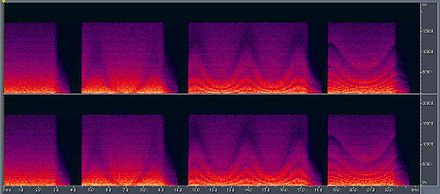
\includegraphics[width=0.75\textwidth]{pic-phaser-03}
  \caption{Результат применения фейзера}
  \label{pic-phaser-03}
\end{figure}

Также фэйзером называют соответствующее устройство. По принципу работы схож с хорусом и отличается от него временем задержки (1-5 мс). Помимо этого задержка сигнала у фэйзера на разных частотах неодинакова и меняется по определённому закону.

Электронный эффект фейзер создается путем разделения звукового сигнала на два потока. Один поток обрабатывается фазовым фильтром, который изменяет фазу звукового сигнала, сохраняя его частоту. Величина изменения фазы зависит от частоты. После микширования обработанного и необработанного сигналов, частоты, находящиеся в противофазе, погашают друг друга, создавая характерные провалы в спектре звука. Изменение отношения оригинального и обработанного сигнала позволяет изменить глубину эффекта, причем максимальная глубина достигается при отношении 50%.

\begin{figure}[h!]
  \centering
  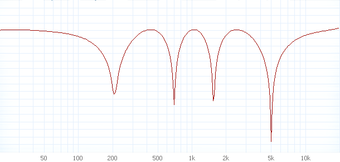
\includegraphics[width=0.75\textwidth]{pic-phaser-01}
  \caption{Спектрограмма сигнала, пропущенного через 8-каскадный фильтр без обратной связи, отношение обработанного и необработанного сигнала: 50/50}
  \label{pic-phaser-01}
\end{figure}

\begin{figure}[h!]
  \centering
  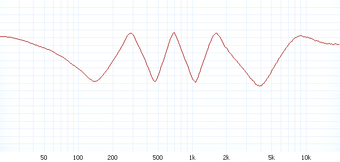
\includegraphics[width=0.75\textwidth]{pic-phaser-02}
  \caption{Спектрограмма сигнала, пропущенного через 8-каскадный фильтр с 50$\perp$ обратной связью, отношение обработанного и необработанного сигнала: 50/50}
  \label{pic-phaser-02}
\end{figure}

Эффект фэйзера подобен эффектам фланжера и хоруса, которые также используют добавление к звуковому сигналу его копий, подаваемых с определенной задержкой (т. н. линию задержки). Однако в отличие от фланжера и хоруса, где величина задержки может принимать произвольное значение (обычно от 0 до 20 мс), величина задержки в фэйзере зависит от частоты сигнала и лежит в пределах одной фазы колебания. Таким образом, фэйзер можно рассматривать как частный случай фланжера.

Эффект имеет следующие параметры:
\begin{itemize}
  \item Глубина (\textit{depth})~--- характеризует диапазон изменения времени задержки.
  \item Скорость (\textit{speed}, \textit{rate})~--- быстрота изменения "<плавания"> звука, регулируется частотой низкочастотного генератора.
  \item Форма волны генератора низкой частоты (\textit{LFO waveform}).
  \item Баланс (\textit{balance}, \textit{mix}, \textit{dry/wet})~--- соотношение необработанного и обработанного сигналов.
\end{itemize}

Фейзер используют для достижения "<синтезации"> или "<электронизации"> натуральных звуков, таких как человеческая речь. В частности, этот эффект популярен в кино- и теле-продукции, где используется для преобразования голоса человека в голос компьютера. Так, например, голос персонажа C-3PO из фильма Звездные войны был создан путем редактирования голоса актера фэйзером. Причина такого использования состоит в том, что спектр звука, что дает фэйзер, является слишком нетипичным для природных звуков.

Фэйзер широко используют также и электрогитаристы, в частности Эдди ван Хален (\textit{Eddie Van Halen}), который использовал фейзер вместе с другими эффектами, после эффекта дисторшн. Многие клавишные инструменты, такие как клавинет, также используют фэйзер для смягчения звуков.

Диалоговое окно \textit{Phaser} открывается командой \textit{Effects > Modulation > Phaser}. Данный эффект может применяться для создания нереальных звуковых эффектов.
В \textit{Adobe Audition} эффект реализован следующим образом: имеется группа фильтров, которые сдвигают фазу сигнала до и после частоты среза. При применении эффекта фильтры периодически переключаются.

\begin{figure}[h!]
  \centering
  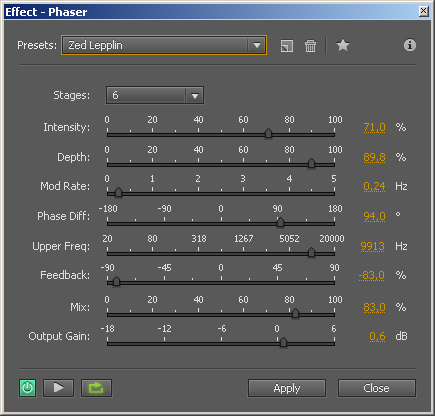
\includegraphics[width=0.75\textwidth]{pic-auphaser-01}
  \caption{Окно эффекта фейзера}
  \label{pic-auphaser-01}
\end{figure}

Параметры фэйзера:
\begin{itemize}
  \item Stages~--- количество фильтров, сдвигающих фазу;
  \item Intensity~--- процент применения эффекта;
  \item Depth~--- глубина модуляции;
  \item Mod Rate~--- частота модуляции;
  \item Phase Diff~--- задает разность фаз стереоканалов.
  \item Upper Freq~--- задает верхнюю частоту среза для фильтров.
  \item Output Gain~--- величина усиления после применения эффекта.
\end{itemize}

Эффект \emph{Enigma} (рис. \ref{pic-enigma-01}), входящий в пакет \emph{Waves}, можно описать как сложный фэйзер/фланжер с реверберацией и обратной связью со сложной фильтрацией, а также дополнительной модуляцией.

\begin{figure}[h!]
  \centering
  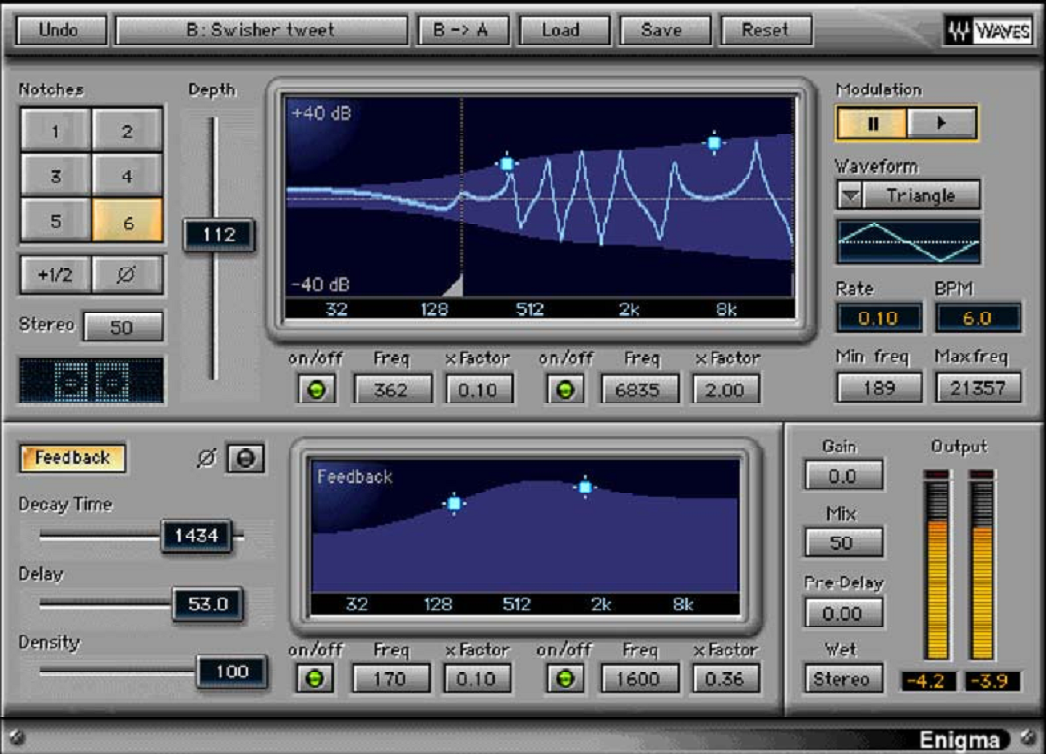
\includegraphics[width=0.75\textwidth]{pic-enigma-01}
  \caption{Окно эффекта \emph{Waves Enigma}}
  \label{pic-enigma-01}
\end{figure}

Окно эффекта содержит четыре основных секции:
\begin{itemize}
  \item вырезы ("<enigma processor">) с опциями фильтрации;
  \item модулятор, который модулирует только процессор вырезов;
  \item обратная связь с опциями фильтрации;
  \item глобальная секция.
\end{itemize}

Секция вырезов (рис. \ref{pic-enigma-02}) содержит следующие элементы управления:
\begin{enumerate}
  \item \emph{Notches} (вырезы)~--- выберите от 2 до 12 (от 1 до 6 пар) вырезов/частотных развёрток.
  \item кнопка $+1/2$ добавляет "<половину пары"> вырезов в верхнюю часть.
  \item \emph{Depth} (глубина)~--- управляет глубиной вырезов в процессоре \emph{Enigma}.
  \item \emph{Stereo} (стерео)~--- управляет как стерео, так и тембральными аспектами процессора.
\end{enumerate}

\begin{figure}[h!]
  \centering
  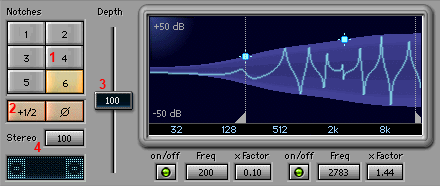
\includegraphics[width=0.5\textwidth]{pic-enigma-02}
  \caption{Секция вырезов эффекта \emph{Waves Enigma}}
  \label{pic-enigma-02}
\end{figure}

 Секция модуляции (рис. \ref{pic-enigma-03}) содержит следующие элементы управления:
 \begin{enumerate}
   \item Вкл/Выкл~--- удобный способ остановить раздражающую модуляцию, "<заморозить"> вырезы при определенном тембре, автоматизировать модулятор.
   \item Sync (синхронизация)~--- при выборе ручной синхронизации (Manual) скорость модулятора устанавливается полностью вручную. При выборе автоматической синхронизации (Auto) скорость модулятора соответствует темпу проекта, и параметры скорости перестают быть доступными, доступен только множитель.
   \item Waveform (форма сигнала)~--- выберите форму сигнала для модулятора. Это меню включает в себя формы: пилообразную вверх, пилообразную вниз, треугольную, синусообразую, квадратную (50\% импульса).
   \item Множитель~---- этот элемент управления выступает в качестве множителя до значения скорости модуляции в параметре \emph{Rate}. Он представляет собой количество циклов в такт. Это верно когда \emph{Rate} установлено внутри или управляется внешне темпом проекта. Фактическая скорость модуляции это значение \emph{Rate} умноженное на значение, установленное в Множителе. (\emph{Скорость модуляции} = \emph{Rate} х \emph{Множитель}).
   \item Rate/BPM (скорость/темп)~--- управляет модуляцией в секундах или ударах в минуту.
   \item MinFreq/MaxFreq (минимальная частота/максимальная частота)~--- устанавливает границы частотного диапазона для развёртки.
 \end{enumerate}

\begin{figure}[h!]
  \centering
  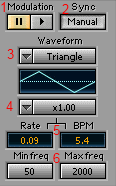
\includegraphics[width=0.2\textwidth]{pic-enigma-03}
  \caption{Секция модуляции эффекта \emph{Waves Enigma}}
  \label{pic-enigma-03}
\end{figure}

 Секция обратной связи (рис. \ref{pic-enigma-04}) содержит следующие элементы управления:
 \begin{enumerate}
   \item Decay time (время затухания)~--- времени затухания сигнала обратной связи.
   \item Delay (задержка)~--- время задержки обратной связи.
   \item Вкл./выкл. обратной связи и кнопка фазы.
   \item Density (плотность)~--- параметр управляет плотностью и стерео разделением отдельных задержек. Когда плотность больше нуля, время задержки для левого и правого каналов будет разной, когда ноль, тогда они будут одинаковыми (таким образом это будет моно).
 \end{enumerate}

\begin{figure}[h!]
  \centering
  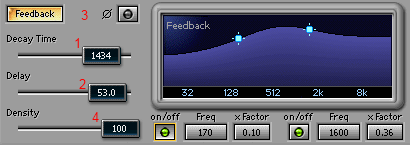
\includegraphics[width=0.5\textwidth]{pic-enigma-04}
  \caption{Секция обратной связи эффекта \emph{Waves Enigma}}
  \label{pic-enigma-04}
\end{figure}

Глобальная секция содержит следующие элементы управления:
\begin{itemize}
  \item \emph{Gain} (усиление)~--- усиление выходного сигнала;
  \item \emph{Mix} (подмешивание)~--- управление балансом между обработанным и не обработанным сигналами;
  \item \emph{Pre-delay} (предварительная задержка)~--- задержки обработанного сигнала перед смешением с сухими.
  \item \emph{Wet} (обработанный)~--- предлагает три режима:
  \begin{enumerate}
    \item \emph{Stereo} (стерео)~--- это стандартный стерео выход обработанного сигнала;
    \item \emph{Mono} (моно)~--- суммирование левого и правого каналов обработанного сигнала;
    \item Mono\emph{ + PhaseReverse} (моно + инвертированная фаза)~- инвертирует фазу левого канала, а затем суммирует его с правым, в результате этого производятся сильный эффект вырезов.
  \end{enumerate}
\end{itemize}

\section{Фазовые преобразования}
В программах цифровой обработки звука есть несколько средств, предназначенных для изменения стерео образа звука:
\begin{itemize}
  \item преобразования моно в стерео и обратно,
  \item расширения стерео-панорамы,
  \item имитации вращения стереополя вокруг слушателя и т.д.
\end{itemize}

В \textit{Adobe Audition} к эффектам подобного назначения относятся:
\begin{itemize}
  \item \textit{Center Channel Extractor}~--- извлечение/удаление центрального канала;
  \item \textit{Graphic Phase Shifter}~--- инструмент для изменения фаз частотных составляющих сигнала.
\end{itemize}

Команда меню \textit{Effects > Stereo Imagery > Center Channel Extractor} вызывает диалоговое окно эффекта (рис. \ref{pic-aucenterchannel-01}), который позволяет сохранять или удалять совпадающие частоты левого и правого каналов (т.е звуков, которые панорамированы в центр: голос, бас и партии главных инструменты). В результате, данный эффект можно использовать для поднятия уровня голоса, баса, ударных, либо для их удаления и создания эффекта karaoke.

\begin{figure}[h!]
  \centering
  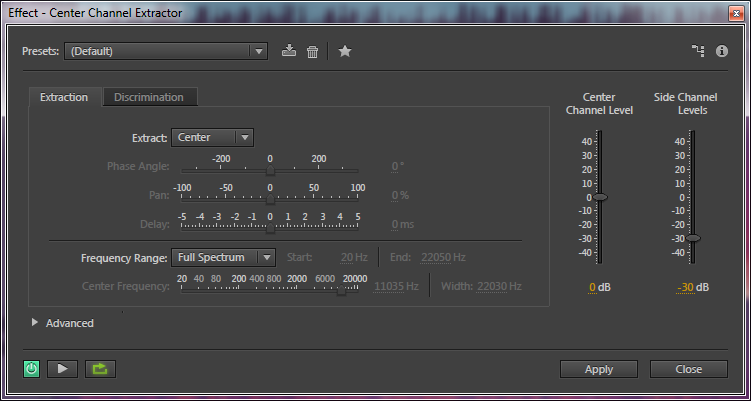
\includegraphics[width=0.75\textwidth]{pic-aucenterchannel-01}
  \caption{Окно эффекта \emph{Center Channel Extractor}}
  \label{pic-aucenterchannel-01}
\end{figure}

Для применения эффекта необходимо определить, какой канал следует удалить (параметр \emph{Extract}), разность фаз (\textit{Phase Angle}), ширину cтереопанорамы (\textit{Pan}) и время задержки (\textit{Delay}). \textit{Frequency Range} определяет полосу частот, в которой будет производиться действие эффекта (имеются шаблоны "<Мужской голос">, "<Женский голос">, "<Бас">, "<Весь спектр">). Слайдером \textit{Center Channel Level} задается усиление центрального канала, а \textit{Side Channel Level}~--- боковых. Слайдер \textit{Crossover Bleed} задает в процентах, сколько из отсекаемых аудио данных эффект будет пропускать в обработанный звук. Параметр \textit{Phase Discrimination} задает разность фаз. Для извлечения центрального канала следует устанавливать большие значения, для удаления~--- небольшие. Рекомендуемые значения от 2 до 7. Рекомендуемые значения \textit{Amplitude Discrimination} = 0,5... 10; \textit{Amplitude Bandwidth} = 1... 20. Параметр \textit{Spectral Decay Rate} следует устанавливать в 0\% для более быстрой обработки, а значения от 80\% до 98\%~--- для полного избавления от фоновых искажений.

Команда меню \textit{Effects > Stereo Imagery > Graphic Phase Shifter} вызывает диалоговое окно эффекта (рис. \ref{pic-auphaseshift-01}), позволяющего вручную задать график зависимости изменения фазы спектральных составляющих сигнала в зависимости от частоты.

\begin{figure}[h!]
  \centering
  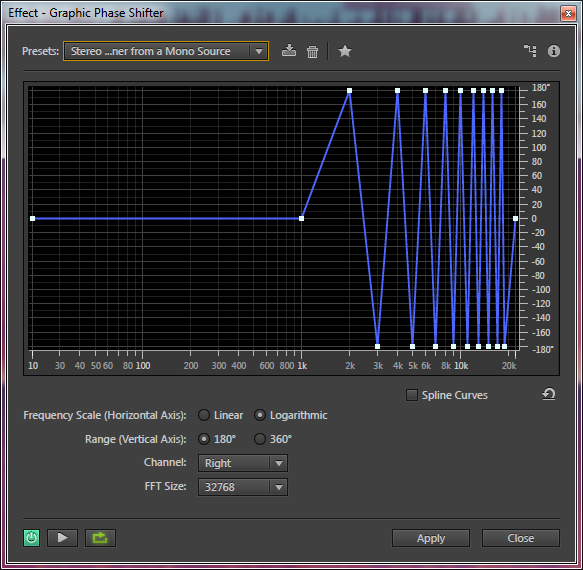
\includegraphics[width=0.5\textwidth]{pic-auphaseshift-01}
  \caption{Окно эффекта \emph{Graphic Phase Shifter}}
  \label{pic-auphaseshift-01}
\end{figure}

Элементы управления позволяют задать масштаб горизонтальной оси (\emph{Frequency Scale}), диапазон значений вертикальной оси (\emph{Range}), выбрать канал (левый, правый или оба), задать параметр \emph{FTT Size} (количество отсчетов для алгоритма БПФ) и включить сглаживание графика.

\section{Другие эффекты}
\subsection{Питч-шифтер}
\textbf{Питч-шифтер} (англ. \textit{pitch shifter})~--- звуковой эффект или соответствующее устройство, добавляющее к сигналу его копию, отстоящую от основного тона на любой интервал в пределах двух октав вверх или вниз.

Реализация эффекта является очень сложной задачей, поэтому в недорогих устройствах могут появляться некоторые проблемы, связанные с потерей качества звучания дополнительного голоса. Другой недостаток связан с появлением небольшой задержки, требуемой устройству для анализа входящего сигнала. Однако в качественных питч-шифтерах указанные недостатки устраняются полностью.

В \emph{Adobe Audition} инструмент \textit{Time And Pitch > Stretch and Pitch} (рис. \ref{pic-austretch-01}) позволяет изменять высоту звука, темп или оба данных параметров одновременно. Данный эффект можно использовать для транспонирования песни (не изменяя темп композиции), или для изменения скорости без изменения высоты тона.

\begin{figure}[h!]
  \centering
  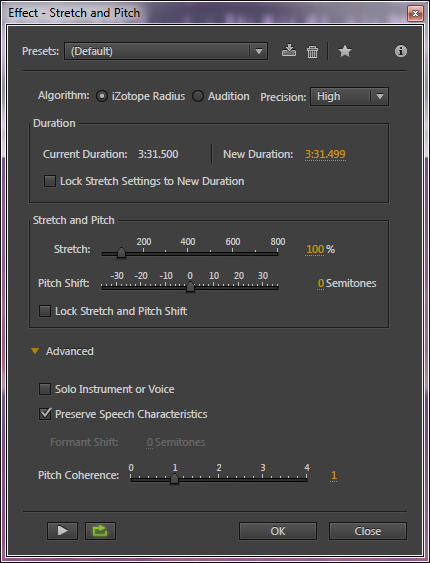
\includegraphics[width=0.5\textwidth]{pic-austretch-01}
  \caption{Окно эффекта \emph{Stretch and Pitch}}
  \label{pic-austretch-01}
\end{figure}

Параметр \textit{Stretch} задает величину растяжения волновой формы (значения меньше 100\% задают сжатие). Параметр \textit{Pitch Shift} позволяет выбрать величину транспонирования высоты звука в полутонах.

\textit{Solo Instrument Or Voice}~--- более точная обработка для соло-инструмента или голоса солиста. \textit{Preserve Speech Characteristics} позволит сохранить реалистичность для голоса. \textit{Formant Shift} определяет, на сколько полутонов будет смещены форманты гласных звуков.

Параметр \emph{Pitch Coherence} управляет изменениями тембра соло-инструмента или вокала. Чем больше значение данного параметра, тем меньше будут слышны артефакты эффекта, но больше будет присутствовать модуляция тона.

~

В \emph{Adobe Audition} при выполнении команды \textit{Time And Pitch > Manual Pitch Correction} редактор переходит в режим \emph{Spectral Pitch Display} (рис. \ref{pic-aupitch-01}) и появляется окно (рис. \ref{pic-aupitch-02}), в котором можно выбрать канал и режим сглаживания огибающей. Сам же эффект позволяет при помощи огибающей задать график изменения высоты тона звука в зависимости от времени.

\begin{figure}[h!]
  \centering
  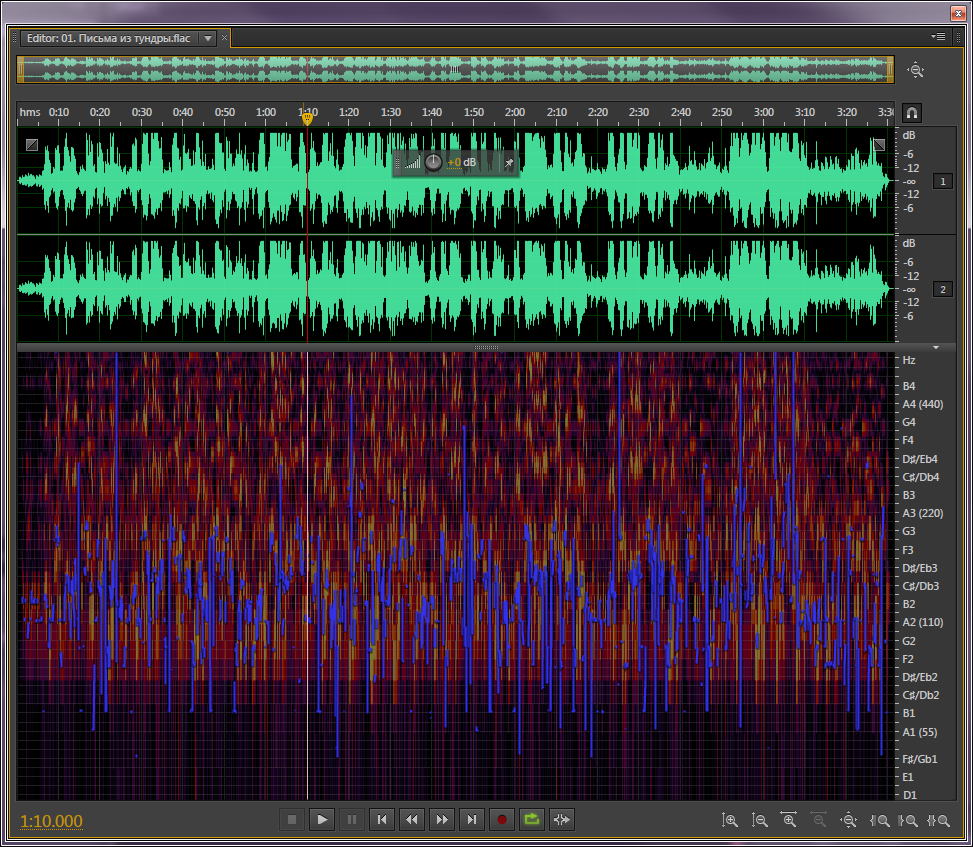
\includegraphics[width=0.75\textwidth]{pic-aupitch-01}
  \caption{Режим \emph{Spectral Pitch Display}}
  \label{pic-aupitch-01}
\end{figure}

\begin{figure}[h!]
  \centering
  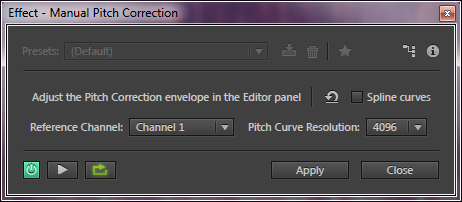
\includegraphics[width=0.5\textwidth]{pic-aupitch-02}
  \caption{Окно эффекта \emph{Manual Pitch Correction}}
  \label{pic-aupitch-02}
\end{figure}

\subsection{Дисторшн и овердрайв}
\textbf{Дисторшн} (англ. \textit{distortion}~---искажение)~--- звуковой эффект, достигаемый искажением сигнала путём его "<жёсткого"> ограничения по амплитуде, или устройство, обеспечивающее такой эффект. Наиболее часто применяется в музыкальных жанрах хард-рок, метал и панк-рок в сочетании с электрогитарой, а также в хардкор-техно и особенно в спидкоре и брейккоре с драм-машиной. Иногда этим термином обозначают группу однотипных звуковых эффектов (овердрайв, фузз и прочие), реализующих нелинейное искажение сигнала. Их также называют эффектами "<перегруза">, а соответствующие устройства~--- "<искажателями">.

Помимо электрогитары эффект применяют и с другими инструментами, например с бас-гитарой. Для бас-гитар применяются особые «искажатели», поскольку "<искажатели"> для гитар, в большинстве случаев, портят басовый звук, срезая значительную часть важных для него низких частот. Альтернативный вариант обработки бас-гитары заключается в использовании обычного "<искажателя"> и смешении чистого и обработанного сигналов в равной пропорции. "<Искажатели"> применяют также для обработки вокала и смычковых инструментов.

Эффект дисторшн, как компонент, присутствует в синтезаторах, эффект-процессорах и компьютерных программах для обработки звука.

\textbf{Овердрайв} (англ. \textit{overdrive} или \textit{перегруз})~--- звуковой эффект, достигаемый искажением сигнала путём его "<мягкого"> ограничения по амплитуде, или соответствующее устройство.

Овердрайв и дисторшн работают по одному физическому принципу~--- ограничение сигнала по амплитуде (рис. \ref{pic-overdrive-01}). В овердрайве это ограничение "<мягкое">, то есть верхушки синусоиды обрезаются не ровной линией, а плавными скруглениями. В дисторшне ограничение "<жёсткое">, то есть верхушки синусоиды просто ровно обрезаются.

Из-за "<мягкого"> ограничения выходной сигнал начинает искажаться пропорционально уровню входного сигнала. Таким образом, при использовании овердрайва для обработки гитарного сигнала можно подчеркнуть динамику звучания. В зависимости от силы удара по струнам будет меняться искажение гитарного сигнала, что кардинально отличается от дисторшна. Дисторшн искажает входной сигнал независимо от его уровня (амплитуды).

\begin{figure}[h!]
  \centering
  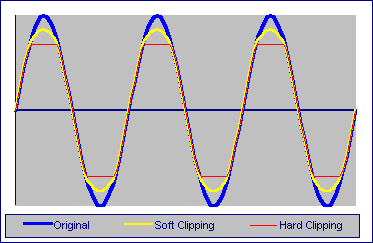
\includegraphics[width=0.75\textwidth]{pic-overdrive-01}
  \caption{Пример сигналограммы с эффектами дисторшн и овердрайв}
  \label{pic-overdrive-01}
\end{figure}

\textbf{Фузз} (более точная транскрипция с английского \textit{Fuzz}~---\textit{Фаз})~--- гитарный эффект, основанный на нелинейном искажении звука электрогитары транзисторными (впоследствии, также цифровыми) устройствами с полной потерей огибающей сигнала.

Фузз появился при попытках получить "<перегруженный"> звук на первых транзисторных гитарных усилителях. Основой эффекта является нелинейное искажение формы сигнала электрогитары. В дальнейшем, звуковой эффект искажения сигнала начал осуществляться двумя путями: подачей слишком высокого уровня сигнала на вход усилительного устройства, которое с разной степенью жёсткости ограничивает и потому сильно искажает сигнал ("<овердрайв"> и "<дисторшн">), или использованием для обработки сигнала транзисторных устройств, жёстко ограничивающих сигнал с практически полной потерей исходного тембра сигнала и ярко выраженным "<органным"> или "<кларнетным"> звучанием (собственно это и есть фузз).

В \emph{Adobe Audition} эффект \emph{Distortion} реализуется в виде особой динамической обработки: к положительным и отрицательным отсчетам применяются различные параметры динамической обработки, что приводит к искажению сигнала (рис. \ref{pic-audistortion-01}). Для каждого графика можно задавать различный режим сглаживания.

\begin{figure}[h!]
  \centering
  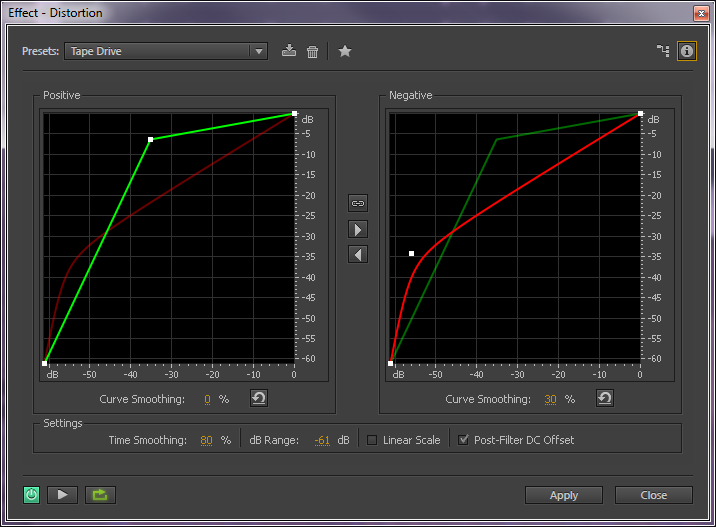
\includegraphics[width=0.75\textwidth]{pic-audistortion-01}
  \caption{Окно эффекта \emph{Distortion}}
  \label{pic-audistortion-01}
\end{figure}

\subsection{Эффект Доплера}
Эффект повторного звучания может быть вызван распространением звука от источника к приемнику различными путями: звук может приходить напрямую и может отразиться от препятствия, находящегося чуть в стороне от прямого пути).

При этом время задержки остается постоянным. В реальной жизни этому соответствует ситуация, когда источник звука, приемник звука и отражающие предметы неподвижны друг относительно друга, при этом частота звука не изменяется.

Если же какой-либо из трех элементов подвижен, то частота принимаемого звука изменяется~--- это проявление \textbf{эффекта Доплера}, который в школьных учебниках традиционно поясняется на примере изменения высоты звучания гудка движущегося паровоза.

Для вызова эффекта в \emph{Adobe Audition} необходимо выполнить команду \textit{Effects > Special > Doppler Shifter} (рис. \ref{pic-audoppler-01}).

\begin{figure}[h!]
  \centering
  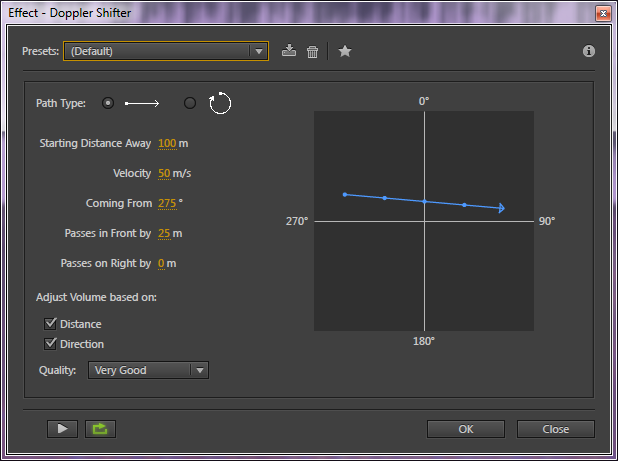
\includegraphics[width=0.75\textwidth]{pic-audoppler-01}
  \caption{Окно эффекта \emph{Doppler Shifter}}
  \label{pic-audoppler-01}
\end{figure}

\textit{Path Type} задает тип пути источника звука:
\begin{itemize}
  \item Straight line (Прямой),
  \begin{itemize}
    \item \textit{Starting distance away}~--- начальное расстояние до источника звука;
    \item \textit{Coming from}~--- направление на источник звука;
    \item \textit{Passing in front by}, \textit{Passing on right by}~--- смещение источника звука.
  \end{itemize}
  \item Circular (По кругу)
  \begin{itemize}
    \item \textit{Radius}~--- радиус вращения источника звука;
    \item \textit{Starting angle}~--- начальный угол вращения;
    \item \textit{Center in front by}, \textit{Center on right by}~--- положение центра вращения.
  \end{itemize}
\end{itemize}

Параметр \textit{Velocity} задает скорость перемещения источника звука.

\end{document}

